\section{Anexos}
\subsection{Carpeta de laboratorio}
\href{https://drive.google.com/drive/folders/1-pCu1uoGqFwTV82Zj6AoLYSWdHQhPP2F?usp=drive_link}{\textbf{Enlace}} de acceso a la carpeta de Google Drive con simulaciones y evidencias del laboratorio.

\subsection{Microcontrolador ATmega328P}\label{Microcontrolador_ATmega328P}

\begin{figure}[H]
  \centering
  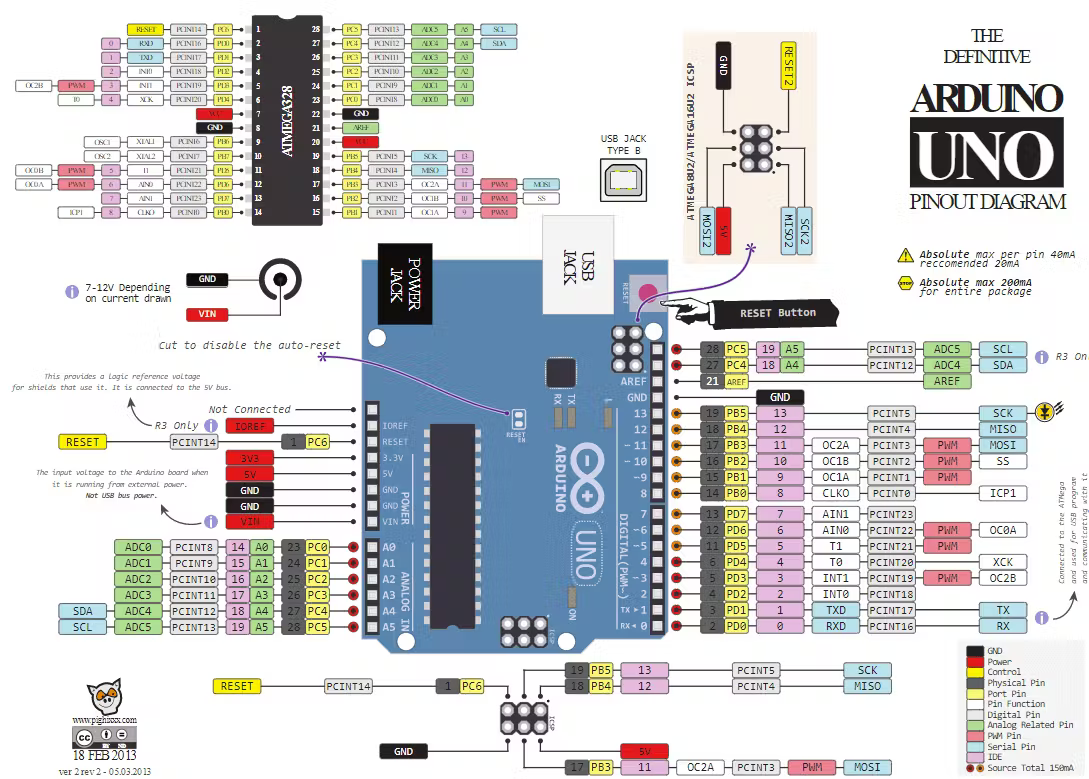
\includegraphics[width=\linewidth]{./Anexos/Full Arduino Pinout.png}
  \caption{Diagrama de pines del Arduino Uno. Fuente: \cite{arduino_uno_pinout}.}
  \label{fig:arduino-uno-pinout}
\end{figure}


\subsection{Matriz de LEDs 1088AS}\label{anexo:Matriz_de_LEDs_1088AS}

\begin{figure}[H]
  \centering
  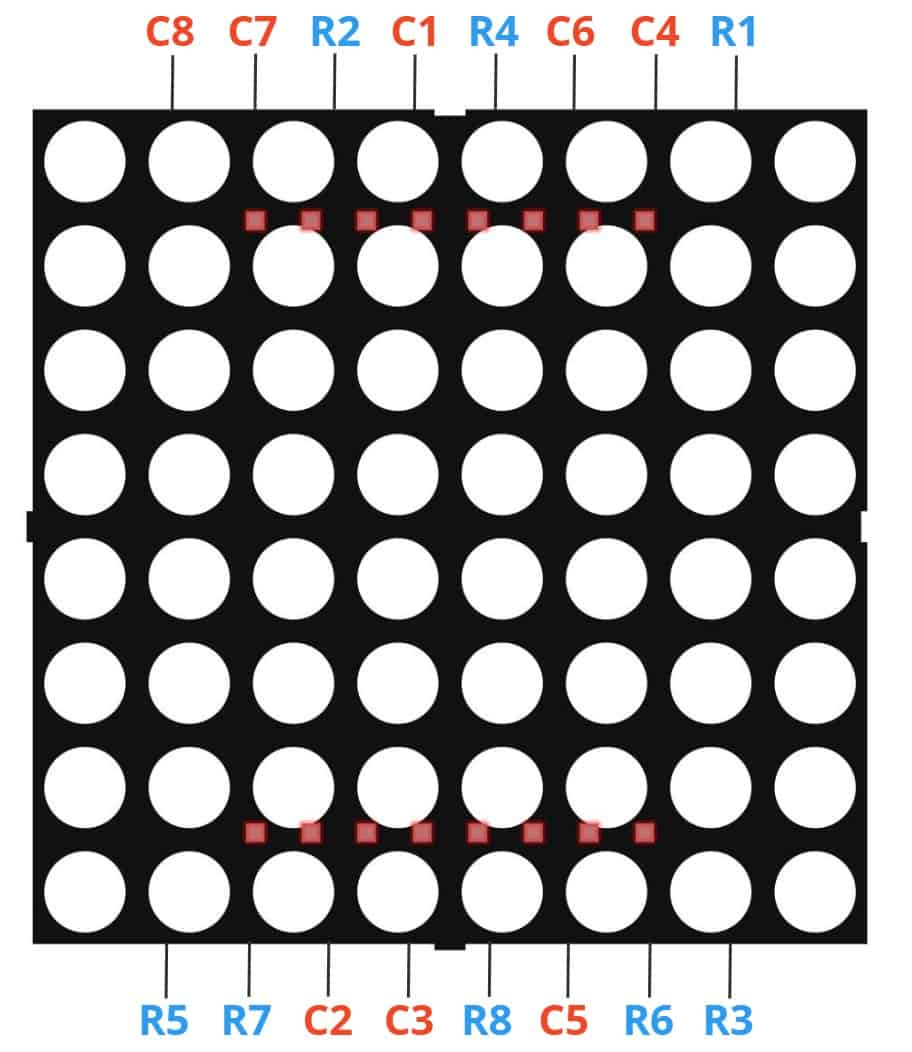
\includegraphics[width=0.7\linewidth]{./Anexos/1088ASPinout.jpg}
  \caption{Pinout de Matriz de LEDs 1088AS. Fuente: \cite{softwareparticles_8x8_arduino}.}
  \label{fig:1088as-pinout}
\end{figure}


\subsection{Comandos Plotter}\label{anexo:Comandos_Plotter}

\begin{figure}[H]
  \centering
  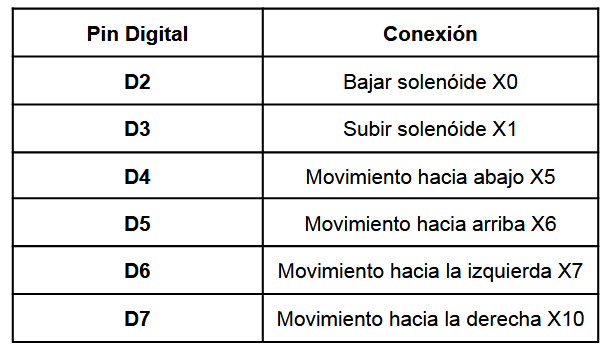
\includegraphics[width=0.9\linewidth]{./Anexos/Comandos Plotter.png}
  \caption{Comandos del Plotter del laboratorio de Mecatrónica. Fuente: Hoja de laboratorio.}
  \label{fig:comandos-plotter}
\end{figure}

\subsection{Señal para conversor digital analogo}\label{anexo:Senal_para_conversor_digital_analogo}
\begin{verbatim}
0x00,0x08,0x10,0x18,0x20,0x28,0x30,0x38,
0x40,0x48,0x50,0x58,0x60,0x68,0x70,0x78,
0x80,0x88,0x90,0x98,0xa0,0xa8,0xb0,0xb8,
0xc0,0xc8,0xd0,0xd8,0xe0,0xe8,0xf0,0xf8,
0xff,0xf7,0xef,0xe7,0xdf,0xd7,0xcf,0xc7,
0xbf,0xb7,0xaf,0xa7,0x9f,0x97,0x8f,0x87,
0x7f,0x77,0x6f,0x67,0x5f,0x57,0x4f,0x47,
0x3f,0x37,0x2f,0x27,0x1f,0x17,0x0f,0x07
\end{verbatim}

\subsection{Stack Pointer}\label{anexo:Stack_Pointer}

Incialización del Stack Pointer:

\begin{verbatim}
RESET:
  cli ldi r16, high(RAMEND)
  out SPH, r16
  ldi r16, low(RAMEND)
  out SPL, r16 sei
  ; ...
\end{verbatim}

Usos del Stack Pointer: rcall, call, interrupciones
preservacion de datos entre subrutinas e ISRs

\subsection{Interrupt service routines}\label{anexo:Interrupt_Service_Routines}

\begin{verbatim}
MI_ISR:
  push r16
  out r16, SREG
  push r16
  ; ... 
  pop r16
  in SREG, r16
  push r16
  reti
\end{verbatim}

\subsection{Delay activo}\label{anexo:Delay_Activo}
\begin{verbatim}
ACTIVE_DELAY:	
  push r18 push r19 push r20

  ldi  r18, 1
  ldi  r19, 10
  ldi  r20, 229
L1: 
  dec  r20
  brne L1
  dec  r19
  brne L1
  dec  r18
  brne L1
  nop

  pop r20 pop r19 pop r18
  ret
\end{verbatim}

\subsection{Vectores de interrupción}\label{anexo:Vectores_de_interrupcion}
\begin{figure}[H]
  \centering
  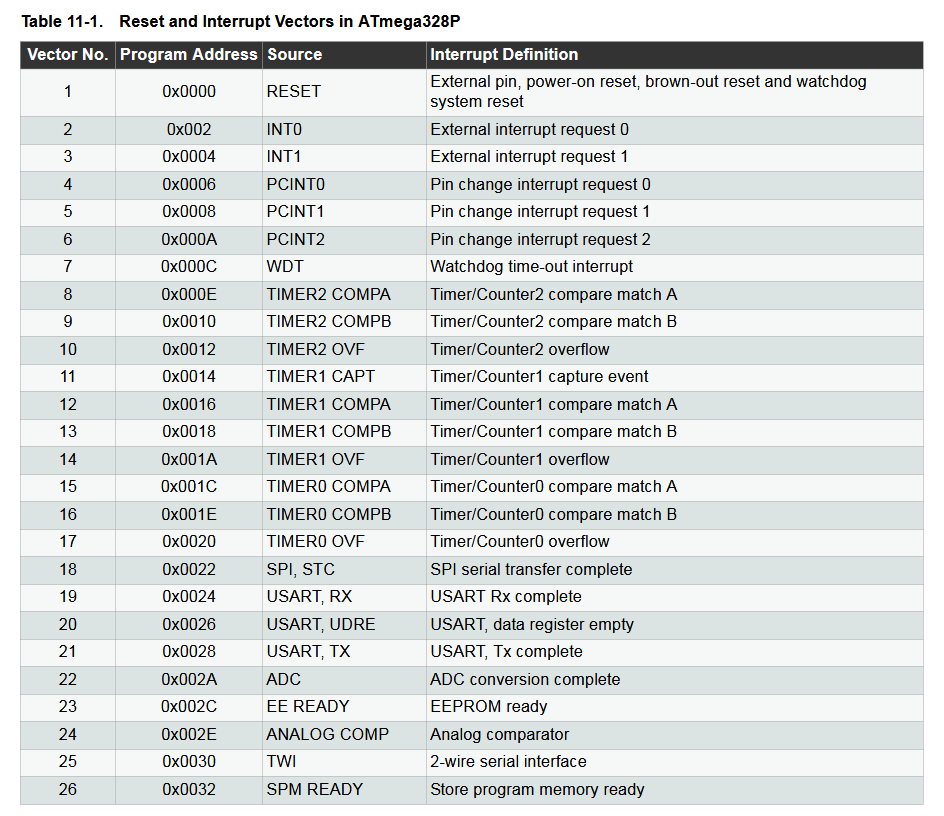
\includegraphics[width=\linewidth]{\detokenize{./Anexos/Marco Teorico/Interrupt Vectors.png}}
  \caption{Vectores de interrupciones en el ATmega328P. Fuente: hoja de datos del ATmega328P\@\cite{atmega328p_datasheet}.}
  \label{fig:interrupt-vectors}
\end{figure}

\subsection{Configuración Timer 1}\label{anexo:Configuracion_Timer_1}

El prescaler del Temporizador 1 es configurado a través del registro TCCR1B el cual posee la siguiente configuración:

\begin{figure}[H]
  \centering
  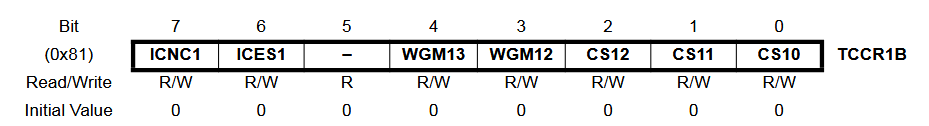
\includegraphics[width=\linewidth]{./Anexos/Marco Teorico/Timers/TCCR1B.png}
  \caption{Registro de control B (TCCR1B) para Timer/Counter1. Fuente: hoja de datos del ATmega328P\@\cite{atmega328p_datasheet}.}
  \label{fig:TCCR1B}
\end{figure}

Los bits CS12 CS11 y CS10 configuran el prescaler del timer conforme a la siguiente tabla: 

\begin{figure}[H]
  \centering
  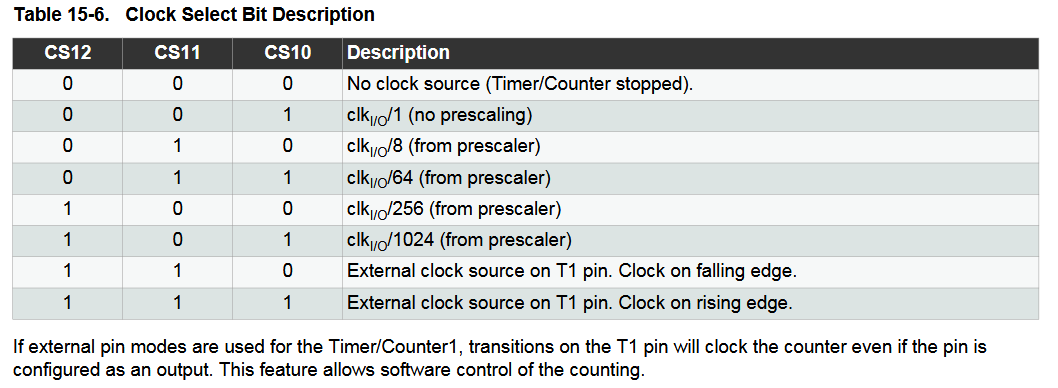
\includegraphics[width=\linewidth]{./Anexos/Marco Teorico/Timers/Prescaler Table.png}
  \caption{Clock Select (CS12:0) opciones de prescaler para Timer/Counter1. Fuente: hoja de datos del ATmega328P\@\cite{atmega328p_datasheet}.}
  \label{fig:prescaler-table}
\end{figure}


El máximo valor de tiempo que admite el Timer 1 (de 16 bits) con el prescaler de 1024 es de 4.19 segundos (aproximadamente). Para valores más grande de delay será necesario crear un contador de overflow aparte utilizando registros de uso general o SRAM

Este es un ejemplo de inicialización de timer 1 para un overflow de 1s

\begin{verbatim}
ldi r16, 0b101       sts TCCR1B, r16
ldi r16, HIGH(49911) sts TCNT1H, r16
ldi r16, LOW(49911)  sts TCNT1L, r16 
\end{verbatim}

El primer registro (TCCR1B) determina el prescaler del reloj (según la figura\ \ref{fig:prescaler-table})

Utilizando la tabla de vectores de interrupcion que se muestra en la figura\ \ref{fig:interrupt-vectors} se mapea el vector de interrupción con la etiqueta del ISR correspondiente:

\begin{verbatim}
.org 0x001A rjmp TIMER1_OVF_ISR

TIMER1_OVF_ISR:
    push r16
    out r16, SREG
    push r16
    ; ... 
    pop r16
    in SREG, r16
    push r16
    reti
\end{verbatim}

\subsection{Interrupciones Externas}\label{anexo:Interrupciones_Externas}
   \subsubsection{EINT}
    Interrupciones externas 

    \begin{figure}[H]
    \centering
    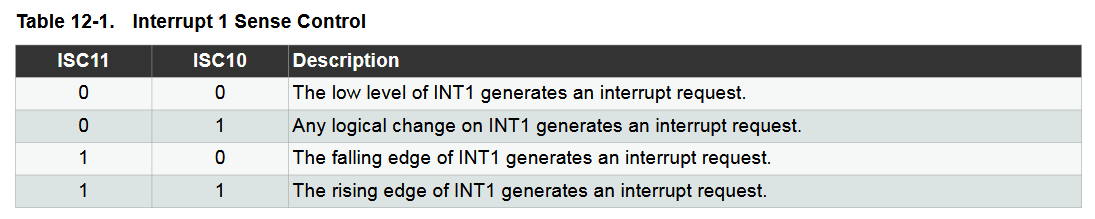
\includegraphics[width=\linewidth]{./Anexos/Marco Teorico/External Interrupts/EICRA table.png}
    \caption{Tabla de configuraciones para EICRA. Fuente: hoja de datos del ATmega328P\@\cite{atmega328p_datasheet}.}
    \label{fig:EICRA-table}
    \end{figure}

    \begin{figure}[H]
    \centering
    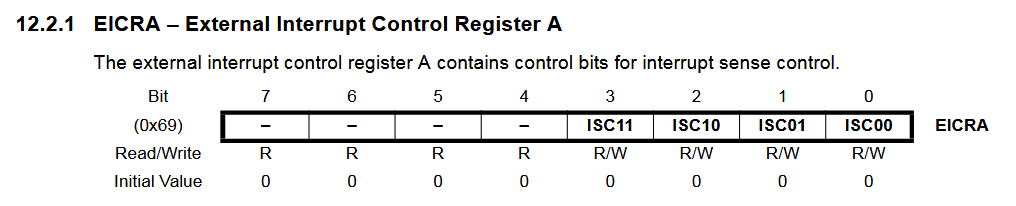
\includegraphics[width=\linewidth]{./Anexos/Marco Teorico/External Interrupts/EICRA.png}
    \caption{Registro de configucación de interrupciones externas EICRA. Fuente: hoja de datos del ATmega328P\@\cite{atmega328p_datasheet}.}
    \label{fig:EICRA}
    \end{figure}

    \begin{figure}[H]
    \centering
    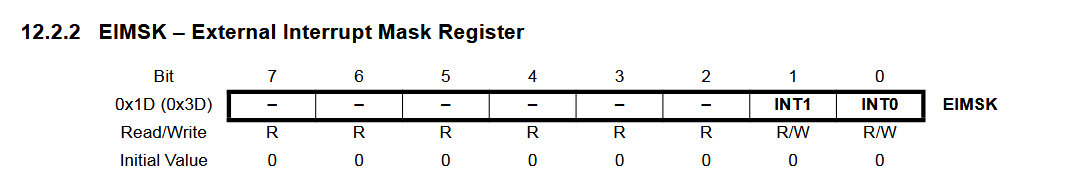
\includegraphics[width=\linewidth]{./Anexos/Marco Teorico/External Interrupts/EIMSK.png}
    \caption{Registro de configucación de máscaras de interrupciones externas EICRA. Fuente: hoja de datos del ATmega328P\@\cite{atmega328p_datasheet}.}
    \label{fig:EIMSK}
    \end{figure}

    \subsubsection{PCINT}
    Interrupciones por cambio en PIN


    \begin{figure}[H]
    \centering
    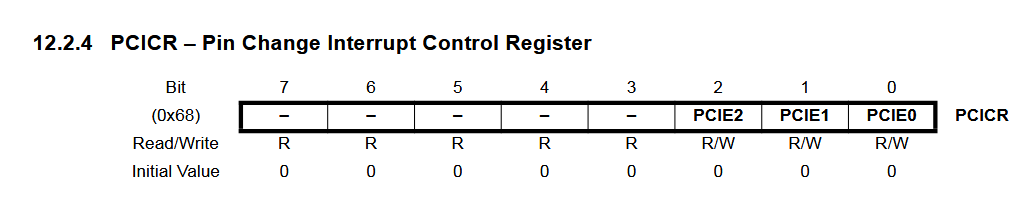
\includegraphics[width=\linewidth]{./Anexos/Marco Teorico/External Interrupts/PCICR.png}
    \caption{Registro de configucación interrupciones PCICR (PCINT). Fuente: hoja de datos del ATmega328P\@\cite{atmega328p_datasheet}.}
    \label{fig:PCICR}
    \end{figure}

    \begin{figure}[H]
    \centering
    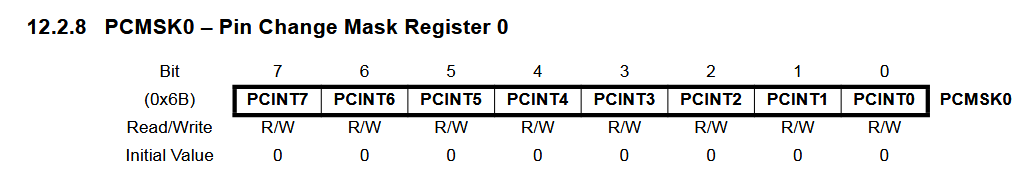
\includegraphics[width=\linewidth]{./Anexos/Marco Teorico/External Interrupts/PCMSK.png}
    \caption{Registro de configucación de mascara de pines para interrupciones PCIMSK0 (PCINT). Fuente: hoja de datos del ATmega328P\@\cite{atmega328p_datasheet}.}
    \label{fig:PCIMSK}
    \end{figure}

\subsection{SRAM}\label{anexo:SRAM}

\begin{verbatim}
.dseg
variable: byte 1  
arreglo: byte 100
\end{verbatim}

% Como leer de sram

\subsection{FLASH}\label{anexo:FLASH}

\begin{verbatim}
.cseg
.org 0x300 TABLA:
    .db 0xFF, 0x30, 0x30, 0xFF
\end{verbatim}

\begin{verbatim}
GET_DATA:
    ldi ZH, high(TABLA<<1)
    ldi ZL, low(TABLA<<1)
    lpm r16, Z+
    ret
\end{verbatim}

% USART

\subsection{USART Asíncrono}\label{anexo:USART_Asincrono}
    \subsubsection{Inicialización}
    \begin{verbatim}
.equ _F_CPU = 16000000
.equ _BAUD = 9600
.equ _BPS = (_F_CPU/16/_BAUD) - 1

.org 0x0024 rjmp USART_RX_ISR

RESET:
; Configurar baudios
sts UBRR0H, high(_BPS)
sts UBRR0L, low(_BPS)

; Habilitar: receptor, transmisor
; e interrupciones por RX
ldi r16, 0b10011000
sts UCSR0B,r16

; Establecer formato:
; 8 data bits, 2 stop bits
ldi r16, (1<<USBS0)|(3<<UCSZ00)
sts UCSR0C,r16

sei
    \end{verbatim}
    \subsubsection{Transmisión}
    \begin{verbatim}
    ldi r16, 0x3f ; Cargar r16 
    sts  UDR0, r16 ; Transmitir
    \end{verbatim}
    \subsubsection{Recepción}

    \begin{verbatim}
    USART_RX_ISR:
    push r16 
    in r16, SREG 
    push r16 

    ; Datos recibidos en r16
    lds r16, UDR0
    ; ...

    pop r16
    out SREG, r16
    pop r16	
    reti
    \end{verbatim}

\subsection{Ring Buffer}\label{anexo:Ring_Buffer}

Reservando RAM para el buffer
\begin{verbatim}
.dseg 
tx_buffer: .byte TX_BUF_SIZE  
tx_head:   .byte 1            
tx_tail:   .byte 1
\end{verbatim}

Tamaño de buffer y máscara de clamping
\begin{verbatim}
.cseg
.equ TX_BUF_SIZE = 16 ; Pot. de 2
.equ TX_BUF_MASK = TX_BUF_SIZE - 1
\end{verbatim}

Avanzar head, y clampear con BUF MASK. Tail se puede avanzar utilizando la mísma lógica
\begin{verbatim}
lds  r17, tx_head
mov  r19, r17 ; Copiar para despues
inc  r19
andi r19, TX_BUF_MASK
\end{verbatim}

El truco de utilizar un múltiplo de 2 y una máscara tiene la ventaja de poder limitar el rango de una variable (clamping) con tan solo una instrucción: ``andi''. 

Si luego de incrementar head, en el caso de que head == tail (buffer lleno), se realiza una espera activa. 
\begin{verbatim}
wait_space: 
; buffer lleno? next == tail
lds  r18, tx_tail
cp   r19, r18
breq wait_space
\end{verbatim}

Guardar un valor en el buffer
\begin{verbatim}
; Z -> Cabeza de buffer
ldi  ZL, low(tx_buffer)
ldi  ZH, high(tx_buffer)
add  ZL, r17 
adc  ZH, r1
st   Z, r16 ; Guardar r16 en buffer
\end{verbatim}

En este caso se decide utilizar una espera activa, pero podría llegar a no ser una buena práctica. Otra alternativa sería simplemente descartar el dato si el buffer está lleno.

    
\subsection{USART Asíncrono con Ring Buffer}\label{anexo:USART_Asincrono_con_Ring_Buffer}

  \subsubsection{Inicialización}
  \begin{verbatim}
.dseg ; Ring buffer ram alocation
tx_buffer: .byte TX_BUF_SIZE  
tx_head:   .byte 1            
tx_tail:   .byte 1           

.cseg
.equ TX_BUF_SIZE = 256
.equ TX_BUF_MASK = TX_BUF_SIZE - 1

.equ _F_CPU = 16000000
.equ _BAUD = 57600 
.equ _BPS = (_F_CPU/16/_BAUD) - 1

; Recieved USART data
.org 0x0024 rjmp USART_RX_ISR	
; USART Data register clear
.org 0x0026 rjmp USART_UDRE_ISR 

RESET:
  clr r1

  ; Stack 
  ldi r16, high(RAMEND) out SPH, r16
  ldi r16, low(RAMEND)  out SPL, r16

  ; Init USART
  ldi r16, low(_BPS)
  ldi r17, high(_BPS)
  rcall USART_INIT

  sei
  ; ...

USART_INIT:	
  sts  tx_head, r1
  sts  tx_tail, r1

  sts UBRR0H, r17
  sts UBRR0L, r16

  ldi r16, 0b10011000
  sts UCSR0B,r16

  ldi r16, (1<<USBS0)|(3<<UCSZ00)
  sts UCSR0C,r16
  ret
    \end{verbatim}
    \subsubsection{Subrutina USART WRITE BYTE}
    \begin{verbatim}
USART_WRITE_BYTE:
  push r17
  push r18
  push r19
  push ZH
  push ZL

  ; head/tail
  lds  r17, tx_head
  lds  r18, tx_tail

  ; r16 -> next = (head + 1) & MASK 
  mov  r19, r17
  inc  r19
  andi r19, TX_BUF_MASK 
  ; Clamping:
  ; Con 256 es 0xFF: no cambia, 
  ; pero deja claro el patrón

  wait_space: 
  ; buffer lleno? next == tail
  lds  r18, tx_tail
  cp   r19, r18
  breq wait_space ; espera activa

  have_space:
  ; Z -> Cabeza de buffer
  ldi  ZL, low(tx_buffer)
  ldi  ZH, high(tx_buffer)
  add  ZL, r17 
  adc  ZH, r1

  st   Z, r16 ; Guardar en buffer

  ; Cabeza = next
  sts  tx_head, r19

  ; Habilitar interrupcion UDRE
  ; así el ISR comienza/continúa 
  ; drenando el buffer
  cli
  lds  r18, UCSR0B
  ori  r18, (1<<UDRIE0)
  sts  UCSR0B, r18
  sei

  pop  ZL
  pop  ZH
  pop  r19
  pop  r18
  pop  r17
ret
\end{verbatim}
    \subsubsection{Interrución USART UDRE ISR}
\begin{verbatim}
USART_UDRE_ISR:
  push r16
  in   r16, SREG
  push r16
  push r17
  push r18
  push r20
  push ZH
  push ZL

  ; r17 = head, r18 = tail
  lds  r17, tx_head
  lds  r18, tx_tail

  ; buffer vacío? head == tail
  cp   r17, r18
  brne usart_udre_send

  ; vacío: deshabilitar UDRIE0
  lds  r20, UCSR0B
  andi r20, ~(1<<UDRIE0)
  sts  UCSR0B, r20
  rjmp usart_udre_exit

  usart_udre_send:
  ; Z -> Cola de buffer
  ldi  ZL, low(tx_buffer)
  ldi  ZH, high(tx_buffer)
  add  ZL, r18
  adc  ZH, r1 

  ; Transmitir byte
  ld   r16, Z
  sts  UDR0, r16

  ; cola = (cola + 1)
  inc  r18                
  andi r18, TX_BUF_MASK 
  ; Clamping:
  ; Con 256 es 0xFF: no cambia, 
  ; pero deja claro el patrón

  sts  tx_tail, r18

  usart_udre_exit:
  pop  ZL
  pop  ZH
  pop  r20
  pop  r18
  pop  r17
  pop  r16
  out  SREG, r16
  pop  r16
  reti
   \end{verbatim}
    \subsubsection{Interrución USART RX ISR}
    \begin{verbatim}
USART_RX_ISR:
  push r16 
  in r16, SREG
  push r16

  ; Leer datos recibidos en r16
  lds r16, UDR0 
  ; ...

  pop r16
  out SREG, r16
  pop r16
  reti
\end{verbatim}


\subsection{Bit Masks}\label{anexo:Bit_Masks}
\subsubsection{SET BIT}
\begin{verbatim}
SET_BIT:	
  push r16
  push r17
  push ZL
  push ZH

  ld  r17, Z     ; read current value
  or  r17, r16   ; set bit
  st  Z, r17     ; write back

  pop ZH
  pop ZL
  pop r17
  pop r16
  ret
\end{verbatim}


\subsubsection{CLEAR BIT}
\begin{verbatim}
CLEAR_BIT:		
  push r16
  push r17
  push ZL
  push ZH

  ld  r17, Z    ; read current value
  com r16       ; invert mask (11110111)
  and r17, r16  ; clear bit
  st  Z, r17    ; write back

  pop ZH
  pop ZL
  pop r17
  pop r16
  ret
\end{verbatim}

\subsection{Look Up Table (LUT)}\label{anexo:Look_Up_Table}
\begin{verbatim}
; Config. de puertos filas
.org 0x310 ROW_PORTS:
  .db 0x25, 0x25, 0x25, 0x25
  .db 0x28, 0x25, 0x28, 0x28

; Config. de pines de puertos
.org 0x320 ROW_MASKS:
  .db 0b00001000, 0b00000010
  .db 0b00010000, 0b00000100
  .db 0b00001000, 0b00100000
  .db 0b00010000, 0b00100000

; Config. de puertos columnas
.org 0x330 COL_PORTS:
  .db 0x2B, 0x2B, 0x2B, 0x28
  .db 0x25, 0x28, 0x28, 0x2B

; Config. de pines de puertos
.org 0x340 COL_MASKS:
  .db 0b00010000, 0b00100000
  .db 0b10000000, 0b00000100
  .db 0b00000001, 0b00000001
  .db 0b00000010, 0b01000000 
\end{verbatim}

\subsection{Máquina de estados}\label{anexo:Maquina_de_Estados}
\begin{verbatim}
.def current_state = r20

STATE_MACHINE:
  cpi current_state, 0
  breq STATE_MACHINE_STATE_0
  cpi current_state, 1
  breq STATE_MACHINE_STATE_1
  cpi current_state, 2
  breq STATE_MACHINE_STATE_2
  cpi current_state, 3

  rjmp STATE_MACHINE_DEFAULT
  

  STATE_MACHINE_STATE_0:
    ; ... state logic
    rjmp STATE_MACHINE_END

  STATE_MACHINE_STATE_1:
    ; ... state logic
    rjmp STATE_MACHINE_END

  STATE_MACHINE_STATE_2:
    ; ... state logic
    rjmp STATE_MACHINE_END

  STATE_MACHINE_DEFAULT:
    ; ... fail state logic
    rjmp STATE_MACHINE_END

  
  STATE_MACHINE_END:
    ; ...
    ret
\end{verbatim}

\subsection{Macros}\label{anexo:Macros}
Definir macros en archivo ``.inc'':

\begin{verbatim}
.macro DISABLE_TIMER_1
	push r16
	ldi r16, 0			 sts TCCR1B, r16
	ldi r16, (0<<TOIE1)	 sts TIMSK1, r16
	ldi r16, (1<<TOV1)   out TIFR1,  r16 
	pop r16
.endmacro

.macro ENABLE_TIMER_1
	; @0 Timer seconds
	push r16
	mov timer1_ovf_counter, @0
	ldi r16, 0b101		 sts TCCR1B, r16
	ldi r16, HIGH(49911) sts TCNT1H, r16
	ldi r16, LOW(49911)	 sts TCNT1L, r16 
	ldi r16, (1<<TOV1)   out TIFR1,  r16 
	ldi r16, (1<<TOIE1)  sts TIMSK1, r16 
	pop r16
.endmacro
\end{verbatim}

Importar macros a ``main.asm'':

\begin{verbatim}
.include "m328pdef.inc"
.include "macros.inc"
\end{verbatim}

